\documentclass[11pt,a4paper]{article}
\usepackage[T1]{fontenc}
\usepackage[utf8]{inputenc}
\usepackage[english]{babel}
\usepackage{amsmath,amssymb,bm}
\usepackage{graphicx}
\usepackage{booktabs}
\usepackage[margin=24mm]{geometry}
\usepackage[hidelinks]{hyperref}
\usepackage{microtype}
\title{Generalized Dynamics and Analytical Criteria for Counterrotation in a Multipole RF Trap}
\author{V17C.14 theory study}
\date{\today}
\begin{document}
\maketitle

\begin{abstract}
We study charged particles interacting through Coulomb forces in a two-family time-dependent multipole field with linear drag and axisymmetric DC confinement. For leading-only RF averaging we derive radial and azimuthal drifts, find locally stable single-particle circular roots with opposite signs for local15 parameters, and formulate exact energy and angular-momentum balances together with analytical approximations for internal ring and axial modes. A published V17C.13 six-particle result is used as a selected reference, not as a basin probability estimate. The results are limited to averaged roots, frozen-phase matrices, and pinned source data: full Floquet/Lyapunov stability, physical feasibility, and stable axial ring separation are not established.
\end{abstract}

\section{Model}
Let \(\tau=\Omega_1t\), \(\bm x_i=\bm r_i/R\), \(\mu_i=m_i/m_1\), \(Q_i=q_i/q_1\), \(\lambda_i=\gamma_i/(m_i\Omega_1)\), \(\kappa=q_1^2/(4\pi\varepsilon m_1R^3\Omega_1^2)\), and \(\phi=q_1\Phi/(m_1R^2\Omega_1^2)\). The N-body equations are
\begin{align}
\bm x_i'&=\bm u_i,\\
\mu_i\bm u_i'&=-Q_i\nabla\phi(\bm x_i,\tau)-\mu_i\lambda_i\bm u_i+
\kappa\sum_{j\ne i}Q_iQ_j\frac{\bm x_i-\bm x_j}{|\bm x_i-\bm x_j|^3}.
\end{align}
The RF potential is represented by Fourier--MFS multipoles and is kept distinct from boundary electrode voltages. The numerical RHS and tangent Jacobian are implemented in `numerical/generalized_dynamics.py`.

The dimensionless energy balance is
\begin{align}
\mathcal E&=\frac12\sum_i\mu_i|\bm u_i|^2+\sum_iQ_i\phi(\bm x_i,\tau)+\kappa\sum_{i<j}\frac{Q_iQ_j}{d_{ij}},\\
\mathcal E'&=\sum_iQ_i\partial_\tau\phi(\bm x_i,\tau)-\sum_i\mu_i\lambda_i|\bm u_i|^2.
\end{align}
Pairwise Coulomb torques cancel in the total angular-momentum balance; RF forcing and drag set the external torque budget.
For a constant-amplitude signed harmonic \(\phi_k=\operatorname{Re}[a\rho^{|k|}e^{i(k\theta-\nu\tau)}]\), \(k\ne0\), the pointwise identity \(Q\partial_\tau\phi_k=(\nu/k)M_k\) holds, where \(M_k=-Q\partial_\theta\phi_k\). A complex envelope \(a(\tau)\) adds \(Q\operatorname{Re}[a'\rho^{|k|}e^{i(k\theta-\nu\tau)}]\). Explicit RF work in the potential-energy balance is distinct from instantaneous mechanical power \((-Q\nabla\phi)\cdot\bm u\).

\section{Local RF averaging}
For a slowly varying position and harmonic acceleration \(\operatorname{Re}[\bm f(\bm X)e^{-i\nu\tau}]\), the linear damped fast response is \(\hat{\bm\xi}=\bm f/(-\nu^2-i\lambda\nu)\). The leading second-order averaged force is
\begin{equation}
\overline{\bm F}_{\rm eff}=\frac12\operatorname{Re}\!\left[(D\bm f)\hat{\bm\xi}^{*}\right].
\end{equation}
For a multipole potential \(\phi=\operatorname{Re}[a\rho^ne^{i(k\theta-\nu\tau)}]\), \(\sigma=\operatorname{sgn}k\),
\begin{equation}
\overline F_\rho=-K_n\rho^{2n-3},\qquad
\overline F_\theta=\sigma K_n\frac{\lambda}{\nu}\rho^{2n-3},\qquad
K_n=\frac{\alpha^2n^2(n-1)|a|^2}{\nu^2+\lambda^2},\quad \alpha=Q/\mu.
\end{equation}
This averaging requires a small local micromotion correction and a slowly varying envelope; \(\epsilon_\mu=1\) is not a universal threshold.
For a finite window of length \(T\) centered at \(\tau_c\), cross terms carry difference- and sum-frequency sinc factors. Near-beat terms must be retained on windows shorter than the beat period, while equal-frequency complex spatial amplitudes must be combined before averaging. Direct finite-window quadrature agrees with the exact sinc expression to a maximum relative difference of \(1.24\times10^{-8}\).

\section{General Multipole Orders and Legacy Candidates}
For modes \((n_j,\sigma_j,\nu_j,a_j)\), define \(S(u)=\sum_jK_ju^{n_j-2}\), \(T(u)=\sum_j(\sigma_jK_j/\nu_j)u^{n_j-2}\), with \(u=\rho^2\). Independent multi-frequency averaging gives circular-root conditions \(\bar\omega=T(u)\) and \(T(u)^2+\alpha\beta-S(u)=0\). Seven requested order pairs were screened for four legacy candidate vectors, retaining each candidate's leading potential coefficients at \(\rho=1\). Stable opposite-sign roots occurred for \((2,3),(2,4),(2,6)\); tested \(p>2\) combinations gave same-sign branches, and \((2,2)\) produced no isolated stable radius. These findings are conditional on the stated amplitude normalization and parameters, not a general multipole-order theorem. Full roots are tabulated in `GENERALIZED_MULTIPOLE_SWEEP_RU.md`.

\section{Local15 circular roots}
For opposite leading harmonics \((n,\sigma)=(2,+1),(4,-1)\), the slow torque and radial balances give
\begin{equation}
\bar\omega(\rho)=K_1-K_2\rho^4/\nu,\qquad
G(\rho)=\bar\omega^2+\alpha\beta-K_1-K_2\rho^4=0,\quad 0<\rho<1.
\end{equation}
The local15 values are \(A=0.03716194907442204\), \(B=0.1626938199343468\), \(\nu=3.1118029452860356\), \(\beta=0.017273303124515367\), \(\lambda_1=0.20975541409005094\), \(\lambda_2=0.12617311138613094\), \(\alpha_1=1\), and \(\alpha_2=0.34126014359705537\). The coupled balance gives \((\rho_1,\bar\omega_1)=(0.5503691530,+0.0014400542)\) and \((\rho_2,\bar\omega_2)=(0.7663818562,-0.0010579232)\). All eigenvalues of the reduced 3D polar Jacobian have negative real parts. This is local stability of an autonomous averaged single-particle system.

The published full-MFS+C V17C.13 reference has group means \(\rho=(0.5480284,0.7660739)\), \(\bar\omega=(+0.0015013354,-0.0009995555)\). It is a selected ordered 3+3 start integrated with RK4/96 for 120,000 RF periods after loading. The 4--6\% frequency differences are cross-model shifts, not controlled numerical errors.

\begin{figure}[ht]
\centering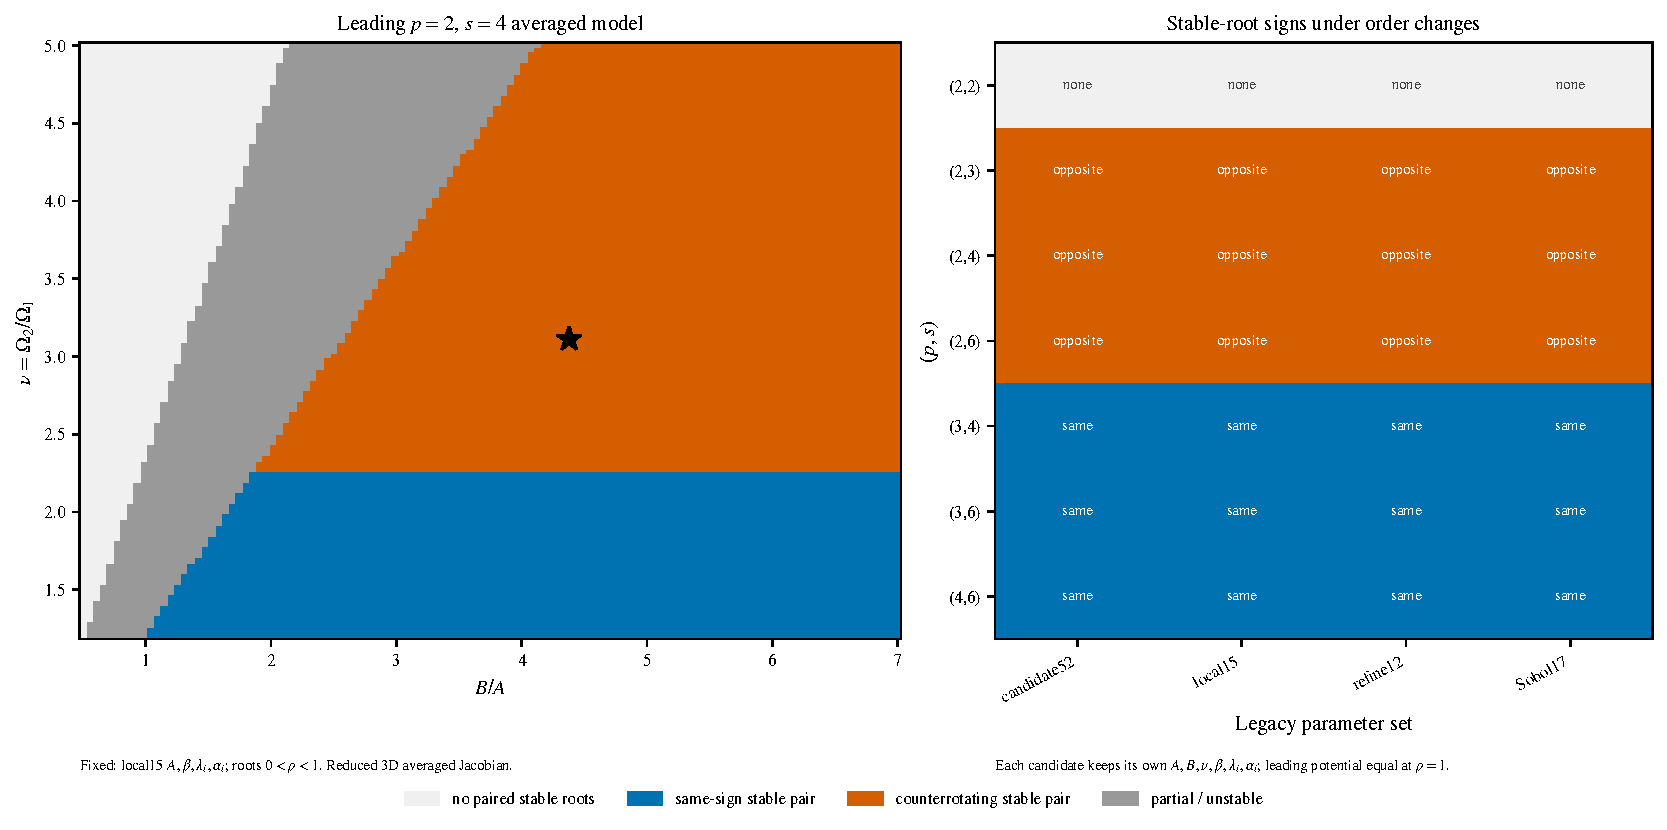
\includegraphics[width=.82\linewidth]{figures/FIG01_ANALYTIC_COUNTERROTATION_MAP.pdf}
\caption{Leading-only phase map and discrete multipole-order check on four legacy candidate vectors. Fixed parameters and classification are documented in the figure and `FIGURE_AUDIT_RU.md`.}
\end{figure}
\begin{figure}[ht]
\centering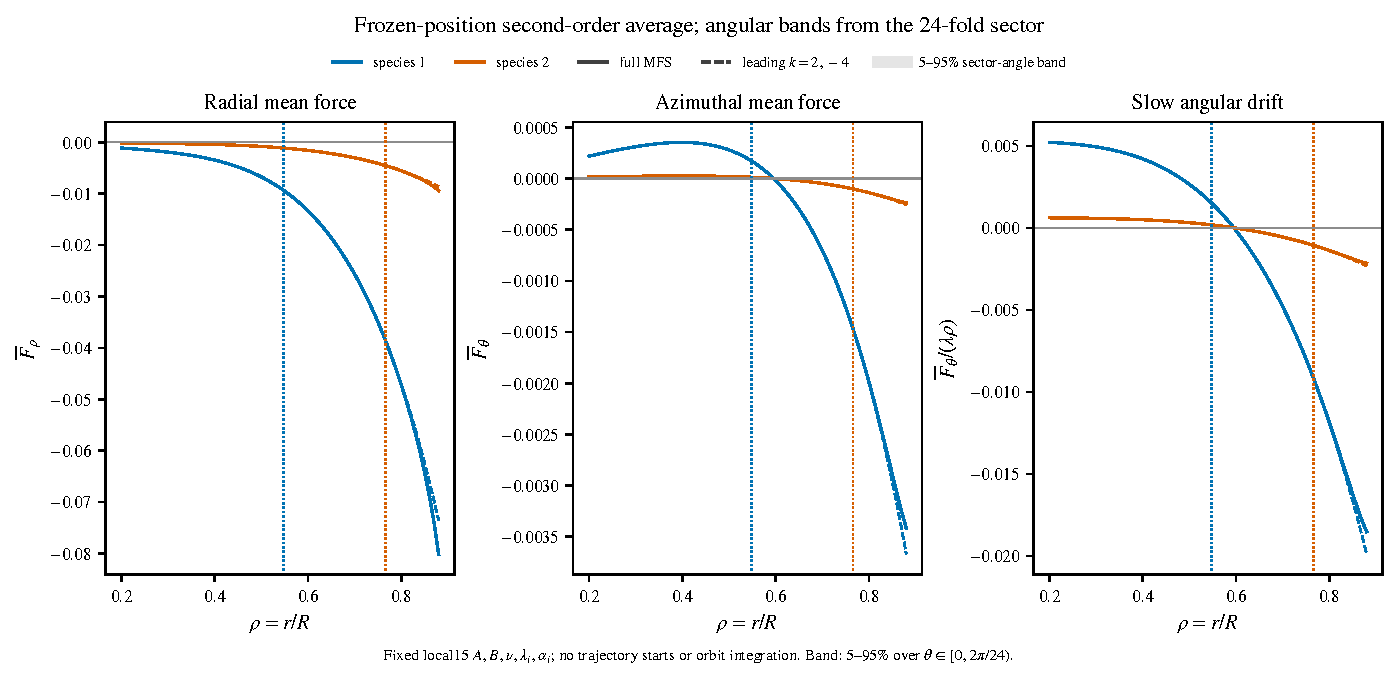
\includegraphics[width=\linewidth]{figures/FIG02_AVERAGED_RF_FORCE_TORQUE.pdf}
\caption{Leading average versus full-MFS frozen-position average across a sector-angle grid.}
\end{figure}
\begin{figure}[ht]
\centering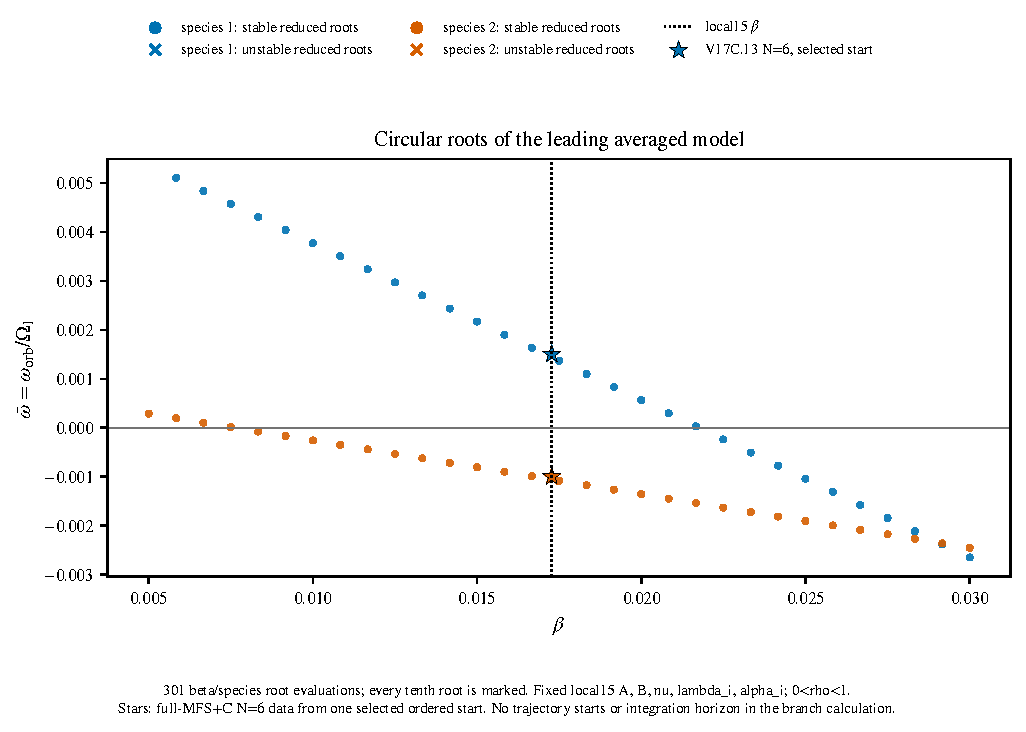
\includegraphics[width=.88\linewidth]{figures/FIG03_ROTATIONAL_BRANCHES.pdf}
\caption{Discrete algebraic circular roots versus \(\beta\); markers classify reduced-model stability and stars show selected full-MFS N=6 means.}
\end{figure}

\section{Torque and collective modes}
The exact RF torque on each particle contains \(-Q_i\partial_{\theta_i}\phi_{\rm RF}\), drag \(-\lambda_iL_i\), and pairwise Coulomb terms. For a triangular ring of three identical particles, the analytical internal phase-mode frequency is
\begin{equation}
\omega_C^2=\frac{5\kappa Q^2}{4\sqrt3\,\mu\rho^3},\qquad
s_\pm=-\lambda/2\pm\sqrt{\lambda^2/4-\omega_C^2}.
\end{equation}
At local15 parameters \(\omega_C/\lambda\simeq0.0174\) and \(0.0180\) at \(C=C_0\); the isolated-ring approximation remains overdamped through \(12C_0\). RF and inter-ring modes are omitted.

In a quadrupole DC field, axial perturbations of a planar 3+3 configuration have a time-varying coefficient matrix whose Coulomb distances depend on relative phase. The frozen-phase Hessian is positive over the sampled phase sector, but this is not a Floquet/Lyapunov test. Adding the fourth-order harmonic
\begin{equation}
H_4=\zeta^4-3\rho^2\zeta^2+\frac38\rho^4
\end{equation}
gives fixed-radius axial extrema at \(\zeta_*^2=3\rho^2/2-\beta_2/(2\beta_4)\). For the local15 radii, \(0.56799<\beta_4/\beta_2<1.10987\) retains central curvature at the inner radius and creates off-axis outer extrema. Full radial and axial stability have not been checked.

\begin{figure}[ht]
\centering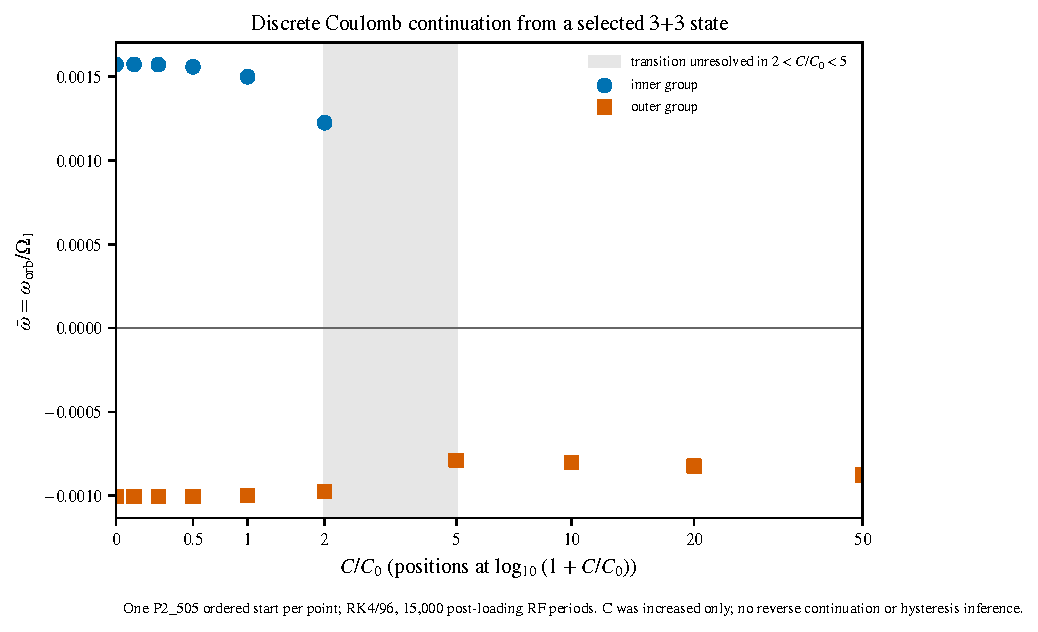
\includegraphics[width=.9\linewidth]{figures/FIG04_COULOMB_ROTATIONAL_TRANSITION.pdf}
\caption{One-way Coulomb sweep with one ordered start per point: the observed sign change is bracketed by \(2<C/C_0\leq5\). The dashed vertical and dotted horizontal lines show the fold and common frequency predicted by the fixed-radius reduced phase model calibrated at \(C=0\); these are not measured boundaries of the full N-body system. This is neither a basin probability nor a hysteresis test.}
\end{figure}
\begin{figure}[ht]
\centering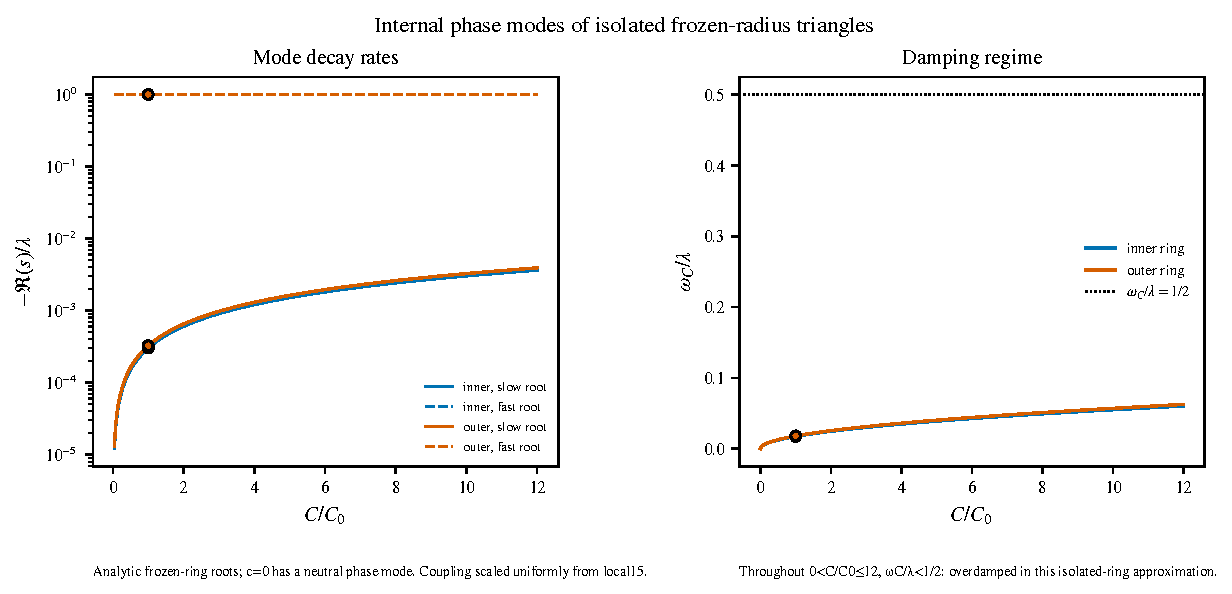
\includegraphics[width=.94\linewidth]{figures/FIG05_INTERNAL_PHASE_MODE_SPECTRUM.pdf}
\caption{Isolated frozen-radius triangular-ring internal phase-mode approximation.}
\end{figure}
\begin{figure}[ht]
\centering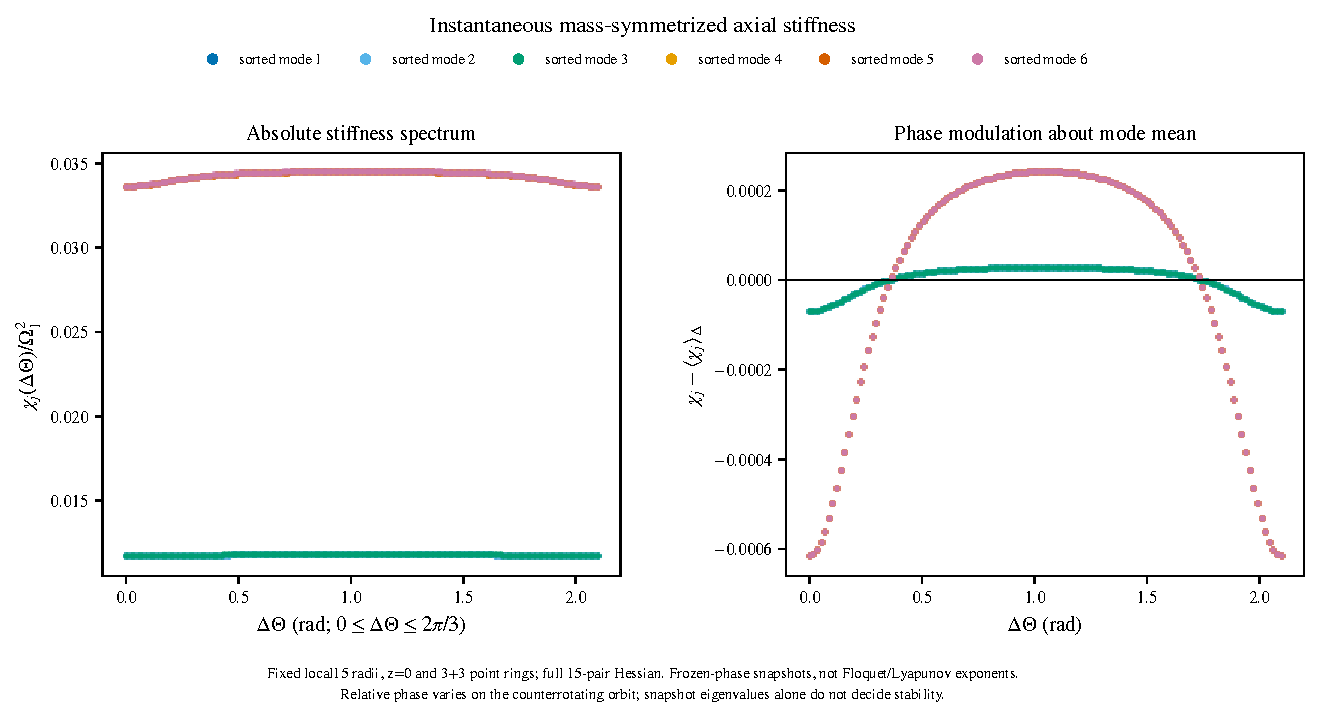
\includegraphics[width=.98\linewidth]{figures/FIG06_AXIAL_COLLECTIVE_STIFFNESS.pdf}
\caption{Instantaneous 3+3 axial stiffness snapshots as relative phase varies; not Floquet exponents.}
\end{figure}
\begin{figure}[ht]
\centering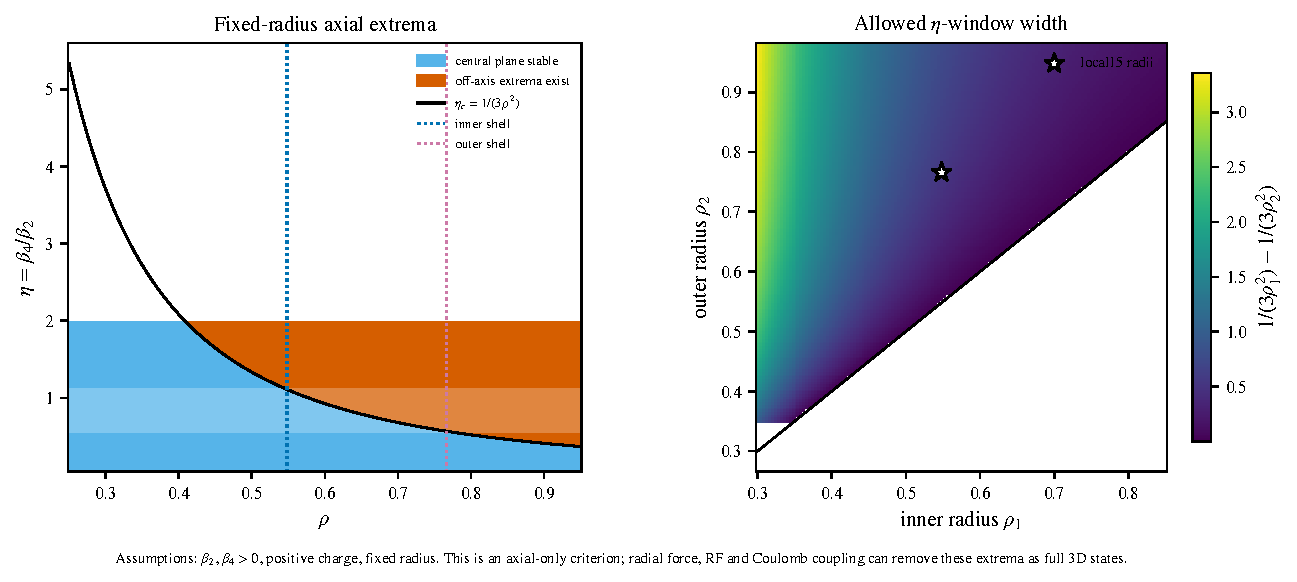
\includegraphics[width=.96\linewidth]{figures/FIG07_H4_AXIAL_STABILITY_MAP.pdf}
\caption{Fixed-radius axial-extrema criteria for the Laplace-compatible \(H_2+H_4\) potential.}
\end{figure}
\begin{figure}[ht]
\centering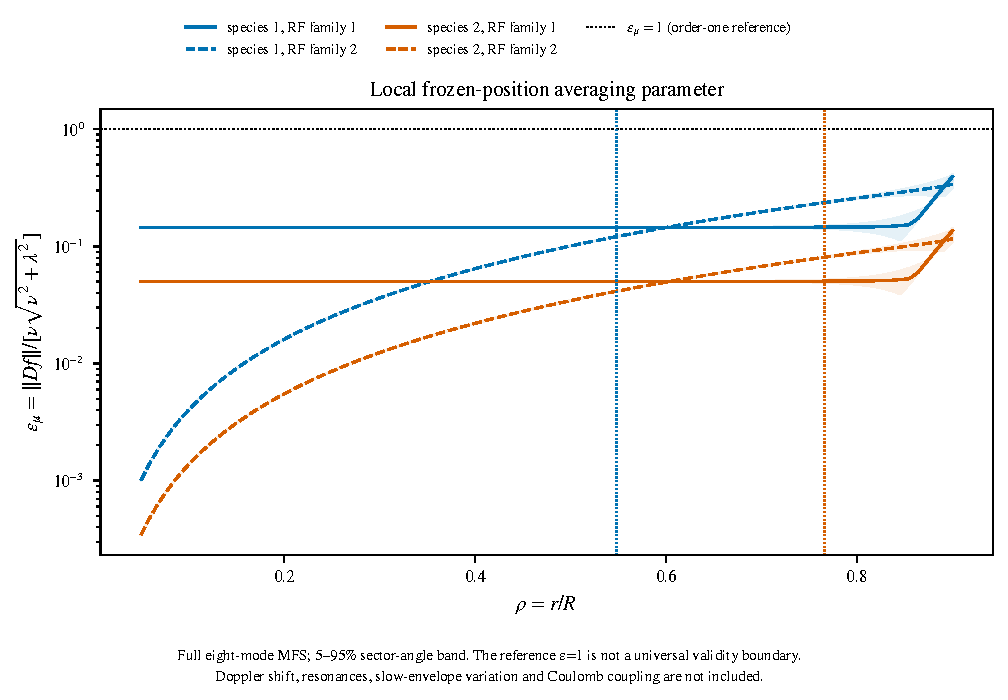
\includegraphics[width=.87\linewidth]{figures/FIG08_AVERAGING_VALIDITY.pdf}
\caption{Local frozen-position micromotion correction indicator; \(\epsilon_\mu=1\) is only an order-one reference.}
\end{figure}

\section{Validation and limits}
Five RHS/Jacobian tests pass. Direct local RF-phase quadrature agrees with the complex-average formula to \(1.5\times10^{-14}\), the leading-mode formula to \(1.1\times10^{-15}\), and the power/torque identity has zero symbolic residual and maximum scaled numerical residual \(8.99\times10^{-16}\). These figures measure local algebra, not trajectory-averaging accuracy. No new trajectory integrations, random starts, RK4 step refinement, DOP853 cross-check, reverse continuation or full tangent/Floquet-Lyapunov calculation were performed. The source audit found the V17C.12B RHS multiplied drag by Cunningham \(C_c\) instead of dividing by it; finalist drag was overstated by 0.153--1.680%, and old capture fractions were not recomputed. Particle sizes, charges, breakdown and gas environment have not received independent qualification in V17C.14. Read all figures together with `FIGURE_AUDIT_RU.md`, `NUMERICAL_VALIDATION_RU.md` and `SOURCE_MODEL_AUDIT_RU.md`.

RF-trap micromotion and Floquet theory are discussed in \cite{Dehmelt1967Storage,Landa2012Modes,Kaufmann2012Eigenmodes}; Coulomb structural transitions in \cite{Dubin1993Structural,Fishman2008Structural}. Rotating-wall Penning plasma experiments \cite{Huang1997Steady,Huang1998PhaseLocked} are contextual analogies only.

\bibliographystyle{unsrt}
\bibliography{references}
\end{document}
